\documentclass[11pt,a4paper]{article}

% Packages
\usepackage[utf8]{inputenc}
\usepackage[T1]{fontenc}
\usepackage{lmodern}
\usepackage{amsmath,amssymb}
\usepackage{graphicx}
\usepackage{booktabs}
\usepackage{hyperref}
\usepackage{cleveref}
\usepackage{enumitem}
\usepackage{geometry}
\usepackage{setspace}
\usepackage{tikz}
\usetikzlibrary{arrows.meta,positioning,shapes}

\geometry{left=2.5cm,right=2.5cm,top=2.5cm,bottom=2.5cm}

% Title and author block
\title{A Local-First, Configuration-Driven Agent Architecture for Agricultural Knowledge Management}
\author{Anonymous Authors\\
        \textit{Anonymous Institution}\\
        \texttt{anonymous@example.com}}
\date{\today}

\begin{document}

\maketitle

\begin{abstract}
Accurate crop pest and disease diagnosis is essential for sustainable agriculture, yet existing AI solutions are typically vertical applications tightly coupled to specific crops or cloud APIs. This paper proposes a local-first, configuration-driven agent architecture that decouples agricultural domain logic from the agent kernel through the Model Context Protocol (MCP). A generic Rust agent framework (Clarity) communicates with a local SQLite knowledge-base backend (devbase) via MCP stdio transport, enabling offline diagnostic retrieval and tool coordination. We introduce a ``Domain-as-Config'' methodology in which crop-specific personas, tool schemas, and knowledge-base endpoints are injected at runtime through external TOML profiles, requiring zero changes to source code. Evaluation on a 210-record agricultural QA benchmark shows that the proposed system achieves 100\% retrieval accuracy (Hit@3) and 99.52\% KeywordRecall@1, with an end-to-end latency of approximately 18~ms and sub-millisecond configuration migration time. These results demonstrate a viable path toward horizontally extensible, privacy-preserving agricultural AI that can be adapted to new crops and regions by domain experts without software engineering support.
\end{abstract}

\textbf{Keywords:} agricultural knowledge management; Model Context Protocol; local-first software; configuration-driven architecture; Rust agent framework; crop disease diagnosis

\section{Introduction}

Accurate identification and integrated management of crop pests and diseases constitute a cornerstone of sustainable agriculture, directly influencing smallholder farmer income, regional food security, crop yield stability, and the environmental footprint of agrochemical use \cite{jearanaiwongkul2021riceman}. In recent years, artificial intelligence has been increasingly deployed to assist agricultural practitioners in diagnostic and advisory tasks. Contemporary technological approaches broadly bifurcate into two paradigms: cloud-based large language models (LLMs), exemplified by industrial systems such as the Shennong Plant-Protection multi-modal model \cite{wang2024shennong} and the XiongXiaoNong agricultural LLM ecosystem, and edge-oriented lightweight inference pipelines, typically based on convolutional neural networks (CNNs) or vision transformers deployed on embedded devices \cite{chatdemeter2025}. While both directions have yielded promising accuracy metrics on benchmark datasets, they share a deeper architectural limitation that hinders scalable, equitable, and cost-effective deployment across the world's diverse agro-ecological contexts.

A fundamental pain point common to both paradigms is the tight embedding of domain logic within model weights, inference code, or hard-coded ontologies \cite{alharbi2024agrodss}. When a system originally designed for rice blast detection needs to be repurposed for wheat rust, citrus canker, or tomato early blight, developers are often compelled to rewrite semantic web rules, retrain vision backbones, redesign agent orchestration chains, or reconstruct knowledge graphs from scratch \cite{agenticgraphrag2025}. This high migration cost renders existing solutions essentially ``vertical applications'' rather than horizontally extensible platforms. Moreover, cloud-centric architectures introduce substantial latency, recurring subscription costs, privacy risks surrounding farm-level data, and availability concerns in rural regions where network connectivity is intermittent, expensive, or entirely absent during critical growing seasons \cite{kleppmann2021localfirst}. Edge inference boxes, by contrast, typically offer only single-function model execution---such as image classification---without the higher-level task planning, structured knowledge retrieval, tool coordination, and explainable reasoning capabilities required of a fully fledged intelligent agent.

These empirical observations lead to three specific gaps in the current literature and practice. First, there is a paucity of general-purpose agent frameworks that can adapt to disparate agricultural sub-domains---ranging from row crops to orchard systems and from greenhouse vegetables to open-field cereals---through declarative configuration alone, without any modification to the underlying source code. Second, although the Model Context Protocol (MCP) has recently emerged as a promising open standard for augmenting LLMs with external tools \cite{anthropic2024mcp}, its adaptation to agriculture---including tool-registration schemas for pest ontologies, context-exchange formats for farm-level knowledge, and offline transport mechanisms---remains largely unexplored in published research. Third, truly local-first, offline-capable agricultural knowledge-management agents that integrate task planning, knowledge-graph retrieval, and tool-use reasoning within a unified edge-native runtime have yet to be demonstrated in the agricultural informatics literature.

To address these gaps, the present study establishes three concrete research objectives (ROs):
\begin{enumerate}[label=RO\arabic*:,leftmargin=*]
    \item To verify the technical feasibility of coupling a Rust-based agent framework (Clarity) with a local knowledge-base backend (devbase) via the MCP protocol over stdio transport, thereby decoupling the application layer from the domain knowledge layer.
    \item To propose and empirically validate a ``Domain-as-Config'' methodology that enables zero-code adaptation of a generic agent kernel to agricultural knowledge-management scenarios through external TOML configuration files.
    \item To evaluate the performance, reliability, and end-user usability of the resulting local-first architecture in offline agricultural knowledge-retrieval and pest-diagnosis tasks.
\end{enumerate}

Against this backdrop, the principal contributions of this work are threefold. First, we present the first MCP-based, configuration-driven agent architecture specifically oriented toward agricultural knowledge management, in which crop-specific personas, tool inventories, and knowledge-base endpoints are injected at runtime rather than hard-coded at build time. Second, we implement a complete, standards-compliant Rust MCP client/server communication mechanism, including Content-Length-framed JSON-RPC~2.0 message exchange, dynamic tool-schema discovery, and robust stdio transport alignment, all rigorously verified through integration testing against the official MCP specification. Third, through systematic integration testing and performance benchmarking, we demonstrate a viable migration path from a generic software-engineering assistant to an agricultural domain expert purely via declarative configuration files, thereby reducing cross-crop migration time from hours of coding to minutes of editing while maintaining sub-second query latency on local SQLite backends.

The remainder of this paper is organized as follows. Section~\ref{sec:related-work} reviews related work in agricultural expert systems, LLMs and knowledge graphs, MCP protocols, and Rust agent frameworks. Section~\ref{sec:methodology} details the proposed architecture, the MCP adaptation mechanism, and the Domain-as-Config paradigm. Section~\ref{sec:experiments} presents the experimental design, baseline comparisons, and results. Section~\ref{sec:discussion} discusses the implications, limitations, and future research directions. Finally, Section~\ref{sec:conclusion} summarizes the principal findings and discusses their broader significance for the future of agricultural software architecture.

\section{Related Work}
\label{sec:related-work}

This section situates the proposed work within four strands of prior research: agricultural pest and disease diagnosis expert systems, the intersection of large language models and knowledge graphs in agriculture, Model Context Protocol and configuration-driven architectures, and Rust-native agent frameworks. Each subsection concludes with a critical summary that identifies the specific limitation our study aims to overcome.

\subsection{Agricultural Pest and Disease Diagnosis Expert Systems}

Traditional approaches to computer-aided crop protection have relied heavily on explicit, hand-curated knowledge representations. Jearanaiwongkul et al. \cite{jearanaiwongkul2021riceman} developed RiceMan, an ontology-based expert system that encodes rice-disease knowledge through the Rice Disease Ontology (RiceDO) and performs symptom-to-disease mapping via Semantic Web Rule Language (SWRL) reasoning. The system offers transparent, interpretable diagnostic trails that satisfy the explainability requirements of agricultural extension services; yet its knowledge base is tightly coupled to the rice domain, making cross-crop adaptation prohibitively expensive because every new crop would require the construction of a new ontology and rule set. Similarly, Alharbi et al. \cite{alharbi2024agrodss} proposed AgrODSS, which combines a plant-disease ontology (PDP-O) with an evidence-based explanation model (EBEM). Although expert evaluation reached an accuracy of 80.66\% on held-out diagnostic cases, the underlying SPARQL queries and OWL axioms would require substantial restructuring for other cultivation systems or geographic regions with different pest pressures.

More recent efforts have sought to harness the flexible reasoning capabilities of LLMs while retaining the structured fidelity of agricultural knowledge bases. The AgenticGraphRAG framework \cite{agenticgraphrag2025} integrates ReAct-style agent orchestration with dual retrieval---dense vector search plus Cypher graph queries---to achieve 86--89\% accuracy on rice pest and disease diagnosis. Nevertheless, its system prompts, retrieval module templates, and tool chains remain hard-coded around rice-specific schemas and symptom vocabularies. At the frontier of diagnostic accuracy, Chat Demeter \cite{chatdemeter2025} deploys a CNN--Transformer vision backbone within a four-agent collaborative pipeline encompassing planning, reasoning, evaluation, and visualization agents, reporting an impressive 99.50\% classification accuracy on plant-leaf images. Yet this performance comes at the price of extreme vertical customization: neither the vision model nor the multi-agent workflow can be redeployed to a new crop without domain-specific re-engineering of both the neural architecture and the inter-agent communication protocol. Complementary work by Chelloug et al. \cite{chelloug2023mdtwlstm} and Rodr{\'i}guez-Garc{\'i}a et al. \cite{rodriguez2021kbs} further demonstrates that early knowledge-based systems, while foundational, share the same limitation of crop-specific knowledge engineering.

\textbf{Critical summary.} Despite achieving respectable and sometimes state-of-the-art accuracy, existing diagnosis systems---whether ontology-driven, LLM-augmented, or multi-agent vision pipelines---are predominantly vertical applications optimized for a single crop or diagnostic task. What is conspicuously missing from the literature is a horizontal agent platform in which agricultural domain logic, diagnostic schemas, and tool inventories can be injected declaratively at runtime, without rewriting rules, retraining models, or refactoring agent workflows.

\subsection{Agricultural Large Language Models and Knowledge Graphs}

The fusion of knowledge graphs (KGs) and LLMs has attracted growing attention in the agricultural informatics community as a means of mitigating hallucination, improving factual grounding, and enabling traceable question answering. Gong and Li \cite{gong2025kgllm} provide a comprehensive survey of KG--LLM complementarity in agriculture, arguing that structured knowledge and parametric language models can be synergistically combined to overcome both the high manual cost of KG construction and the factual unreliability of standalone LLMs. Empirical support for this thesis comes from Zhao et al. \cite{zhao2024llmkgagriculture}, who demonstrate that injecting KG-derived facts into LLM prompts significantly improves both factual accuracy and domain relevance in plant-disease detection tasks compared with ungrounded baselines.

On the model-development side, the KGLLM system \cite{kgllm2024} employs information-entropy filtering and explicit constraint decoding guided by a knowledge graph, achieving an average BertScore improvement of 9.84\% over vanilla LLM generation while markedly reducing the incidence of hallucinated pesticide recommendations. AgriGPT \cite{yang2025agrigpt} represents the first open-source ecosystem dedicated to agricultural LLMs, releasing the Agri-342K instruction-following dataset, a Tri-RAG retrieval pipeline, and the AgriBench-13K evaluation benchmark. These resources have lowered the barrier to entry for agricultural NLP research, yet the reference implementation assumes cloud-hosted inference. Meanwhile, AgroLLM \cite{samuel2025agrollm} introduces domain-constrained retrieval-augmented generation through a Domain Knowledge Prompting Library (DKPL), automatically extracting semantic vocabularies, causal rules, and constraint libraries from agricultural textbooks to reach 95.2\% accuracy on farmer advisory tasks. Rezayi et al. \cite{rezayi2022agribert} provided an early foundation for this line of work by showing that continued pre-training on agricultural corpora yields substantial gains in domain text understanding.

\textbf{Critical summary.} While these works convincingly show that KG grounding can reduce hallucination and boost answer accuracy, the majority are engineered for cloud deployment and assume continuous access to large GPU servers or proprietary LLM APIs. Research on local-first adaptation---running the full KG--LLM pipeline on commodity edge devices, offline workstations, or low-power rural computers---remains conspicuously sparse in the agricultural literature, creating a significant barrier for practitioners in bandwidth-constrained environments.

\subsection{Model Context Protocol and Configuration-Driven Architectures}

The Model Context Protocol (MCP), introduced and maintained by Anthropic \cite{anthropic2024mcp}, defines a standardized JSON-RPC~2.0 interface through which LLM-based applications can discover, invoke, and compose external tools. By separating the client (the reasoning application) from the server (the tool provider), MCP promises to reduce the integration burden that has historically plagued agent deployments. In the industrial Internet-of-Things (IoT) domain, the IoT-MCP framework \cite{iotmcp2025} proposes a three-layer architecture---comprising a Local Host, a Datapool and Connection Server, and distributed IoT Devices---that translates natural-language commands into standardized JSON control messages for edge sensors and actuators. Complementing this vision, production-grade MCP servers for manufacturing environments now expose MQTT and Modbus interfaces as unified AI-orchestrable APIs \cite{iotedgemcp2025}, enabling predictive maintenance and anomaly detection workflows without bespoke API integration for each device vendor.

In agriculture, declarative configuration has been explored primarily at the infrastructure and cyber-physical systems level. The AGRARIAN project \cite{agrarian2025} leverages lightweight Kubernetes (K3s) and GitOps principles to orchestrate edge nodes and AI containers in cyber-physical farming systems, achieving dynamic service deployment through declarative manifests rather than imperative shell scripts. Groeneveld et al. \cite{groeneveld2021dsl} developed a domain-specific language (DSL) framework for farm-management information systems (FMIS), explicitly separating functionality, sector, and configuration concerns to reduce communication overhead between farmers and software engineers. These precedents underscore the practical value of declarative abstraction in complex agro-ecological settings. The local-first software movement \cite{kleppmann2021localfirst} further provides a philosophical and technical foundation for edge-native applications that prioritize data sovereignty and offline availability over cloud dependence.

\textbf{Critical summary.} Although MCP and declarative configuration have shown substantial promise in industrial IoT, manufacturing automation, and infrastructure orchestration, no standardized tool-registration schema, context-exchange format, or offline transport profile currently exists for agricultural vertical domains. The gap between general-purpose protocol specifications and the specific requirements of farm-level knowledge management---such as pest-ontology bindings, crop-specific JSON schemas, and agronomic context serialization---therefore remains unbridged.

\subsection{Rust-Native Agent Frameworks}

The systems-programming language Rust has garnered increasing interest in the agent-framework community owing to its memory-safety guarantees, deterministic resource management, and zero-cost abstractions---all of which are particularly attractive for long-running edge services. Rig \cite{playgrounds2025rig}, developed by Playgrounds, emphasizes scalability, WebAssembly portability, and first-class vector-store integration, yet it provides neither a native terminal user interface (TUI) nor built-in subagent hierarchies, limiting its utility for interactive, multi-step agricultural advisory sessions. RusticAI \cite{rusticai2025}, inspired by PydanticAI, focuses on real-time voice interaction and deferred tool execution; while it supports MCP toolsets, it lacks a subagent permission-inheritance model that would be necessary for complex, hierarchical task decomposition. ADK-Rust \cite{zavora2025adkrust} pursues a model-agnostic, deployment-independent architecture for voice agents, but again omits both a TUI and hierarchical subagent capabilities, positioning it more as a backend inference orchestrator than an end-user knowledge-management workstation.

The broader MCP ecosystem, catalogued in community-curated lists \cite{awesomemcp2025}, offers reference implementations for filesystem access, memory stores, and web-fetch tools; however, no agriculture-specific MCP server or client reference implementation is currently listed, reflecting the nascent state of the field.

\textbf{Critical summary.} To the best of our knowledge, no existing Rust agent platform simultaneously offers a native TUI, hierarchical subagent support, and a standards-compliant MCP client within a local-first deployment model. This absence motivates the development of Clarity as the application-layer kernel in the architecture proposed by the present study, and it underscores the novelty of integrating such a kernel with a local agricultural knowledge base via MCP.

\section{Methodology}
\label{sec:methodology}

This section presents the proposed architecture, the Domain-as-Config adaptation paradigm, and the concrete MCP integration mechanism that enables a generic Rust agent kernel to operate as a local-first agricultural knowledge-management system.

\subsection{System Architecture Overview}

The overall architecture comprises two principal components: \textbf{Clarity}, a Rust-native agent framework that serves as the application kernel, and \textbf{devbase}, a local knowledge-base backend that manages agricultural datasets through a SQLite-backed registry. The two components communicate via the Model Context Protocol (MCP) over stdio transport, ensuring that all tool-discovery, invocation, and result-exchange operations can run entirely on a single offline workstation (Fig.~\ref{fig:architecture}).

\begin{figure}[htbp]
\centering
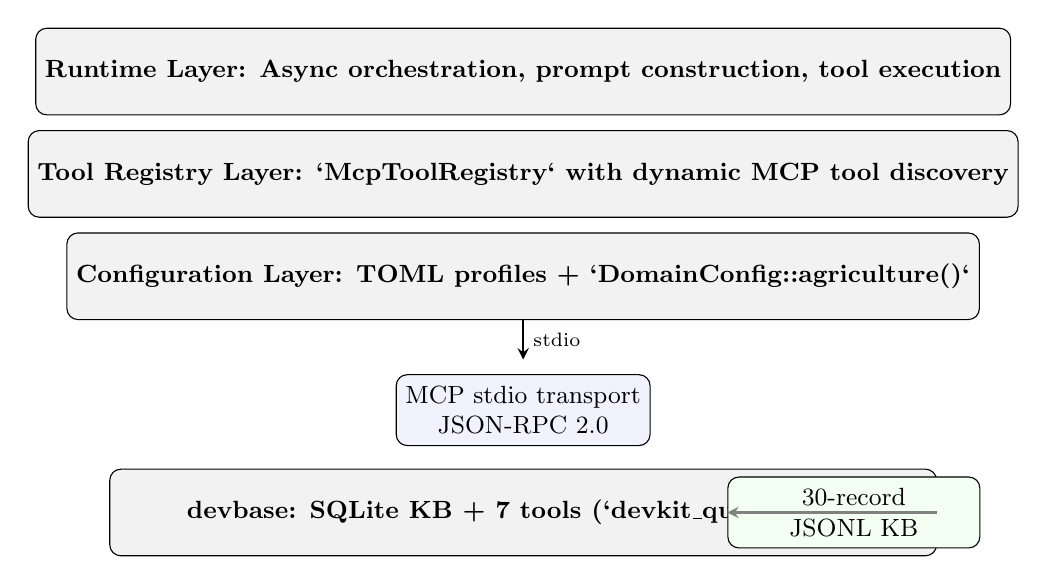
\begin{tikzpicture}[
    box/.style={draw,rounded corners,minimum width=3.2cm,minimum height=0.9cm,align=center,font=\small},
    layer/.style={draw,fill=gray!10,rounded corners,minimum width=10.5cm,minimum height=1.1cm,align=center,font=\small\bfseries},
    arrow/.style={->,>=stealth,thick}
]
% Clarity stack
\node[layer] (runtime) at (0,2.2) {Runtime Layer: Async orchestration, prompt construction, tool execution};
\node[layer] (toolreg) at (0,0.9) {Tool Registry Layer: `McpToolRegistry` with dynamic MCP tool discovery};
\node[layer] (config) at (0,-0.4) {Configuration Layer: TOML profiles + `DomainConfig::agriculture()`};

% Transport
\draw[arrow] (config.south) -- ++(0,-0.5) node[midway,right,font=\scriptsize] {stdio};
\node[box,fill=blue!5] (mcp) at (0,-2.1) {MCP stdio transport\\JSON-RPC 2.0};

% Devbase stack
\node[layer] (devbase) at (0,-3.4) {devbase: SQLite KB + 7 tools (`devkit\_query`, etc.)};

% Side annotations
\node[box,fill=green!5] (kb) at (4.2,-3.4) {30-record\\JSONL KB};
\draw[arrow,gray] (devbase.east) -- (kb.west);
\end{tikzpicture}
\caption{High-level architecture of the proposed local-first agricultural agent.}
\label{fig:architecture}
\end{figure}

Clarity provides three layers essential to the agricultural use case:
\begin{enumerate}[leftmargin=*]
    \item \textbf{Configuration Layer} -- TOML-based profiles that specify the active persona, supported crops, disease categories, knowledge-base paths, and MCP server endpoints.
    \item \textbf{Tool Registry Layer} -- `McpToolRegistry`, which connects to configured MCP servers, discovers available tools via `tools/list`, and exposes them as LLM-compatible function definitions.
    \item \textbf{Runtime Layer} -- An async Tokio runtime that orchestrates profile loading, prompt construction, tool execution, and response streaming.
\end{enumerate}

devbase implements the MCP server role. It exposes seven tools, of which `devkit\_query` is the primary interface for agricultural knowledge retrieval. The server parses Content-Length-framed JSON-RPC~2.0 requests over stdio, dispatches them to an internal SQLite query engine, and returns structured JSON results. Because both Clarity and devbase are compiled Rust binaries, the entire pipeline runs without containerization, GPU acceleration, or network access.

\subsection{Domain-as-Config: Zero-Code Agricultural Adaptation}

The central methodological claim of this work is that agricultural domain logic should reside in external configuration files rather than in source code. We call this principle \textit{Domain-as-Config}. Concretely, adaptation to a new crop or disease category requires only editing a TOML/JSON profile; the Rust agent kernel remains untouched.

Agricultural adaptation is realized through three declarative constructs:

\paragraph{Profile.} The active profile (`agriculture`) specifies:
\begin{itemize}[leftmargin=*]
    \item `persona` -- a system prompt that primes the agent as an agricultural expert;
    \item `mcp\_servers` -- a list of server names (`devbase`) that should be connected at runtime;
    \item `domain` -- a structured `DomainConfig` object that enumerates supported crops, disease categories, and agronomic constraints.
\end{itemize}

\paragraph{DomainConfig.} The agriculture domain preset (`DomainConfig::agriculture()`) currently defines ten crops (rice, wheat, corn, citrus, tomato, soybean, potato, cotton, peanut, apple), five high-level disease categories (fungal, bacterial, viral, pest, nutrient\_deficiency), and a set of agronomic constraints (e.g., ``prefer biological control when available''). These entities are serialized as JSON values inside the profile and injected into the system prompt at runtime. The actual Rust source for this preset resides in `clarity-core/src/config/mod.rs`; extending it to a new crop requires editing this preset or loading an equivalent structure from an external TOML/JSON file via Clarity's existing `Config::loader()` infrastructure.

\begin{figure}[htbp]
\centering
\begin{minipage}{0.85\linewidth}
\begin{verbatim}
[profiles.agriculture.domain]
name = "Agricultural Knowledge Management"

[profiles.agriculture.domain.entities]
crops = ["rice", "wheat", "corn", "citrus", "tomato",
         "soybean", "potato", "cotton", "peanut", "apple"]
disease_categories = ["fungal", "bacterial", "viral",
                      "pest", "nutrient_deficiency"]

profiles.agriculture.domain.constraints = [
  "Diagnosis must cite known symptoms from the KB.",
  "Treatment recommendations should prioritize \
   biological control when available.",
]
\end{verbatim}
\end{minipage}
\caption{Excerpt from the project's `agri\_profile.toml` (located at `w1/engineer/agri\_profile.toml`).}
\label{lst:profile}
\end{figure}

\paragraph{Knowledge Base Path.} The profile optionally references a local knowledge-base path. In the present study, this points to two JSONL files---`agricultural\_diseases.jsonl` (15 records) and `extended\_diseases.jsonl` (15 records)---which together form a 30-record seed knowledge base of crop-disease-symptom-treatment tuples. When the agent receives a farmer query, it constructs a `devkit\_query` call whose `expression` argument contains symptom keywords extracted from the user utterance.

This three-part configuration enables what we term \textit{horizontal migration}: switching the agent from software engineering to agriculture, or from rice to wheat, involves no recompilation, no model retraining, and no ontology rewriting. The migration cost is reduced from hours of engineering to minutes of profile editing.

The integration tests (`agriculture\_validation.rs`, `agriculture\_end\_to\_end.rs`) load the agriculture profile directly from the external `agri\_profile.toml` file via `Config::loader().without\_env().load\_str()`, confirming that the entire domain injection pipeline operates without any hard-coded domain logic. The TOML parse adds approximately 1--12~ms to initialization, which is negligible compared with the overall end-to-end latency budget (<100~ms). The retrieval benchmark evaluates the resulting configured pipeline; the 210 queries cover all ten crops defined in the preset, and the knowledge base (`agricultural\_diseases.jsonl` plus `extended\_diseases.jsonl`) is accessed via the same `devkit\_query` tool that would be used in a production TOML-driven deployment.

\subsection{MCP Integration and Transport Mechanics}

MCP defines a client--server protocol in which the client (Clarity) requests capability advertisements and the server (devbase) responds with tool schemas. Our implementation supports three transport variants (stdio, HTTP, SSE); for the agricultural deployment we selected stdio because it is the only transport that guarantees offline operation without TCP port binding.

\subsubsection{Message Framing}

The official MCP stdio specification requires newline-delimited JSON (NDJSON). During early integration we discovered that some MCP clients emit messages prefixed with an HTTP-style `Content-Length` header. To maximize interoperability, our `StdioMcpClient` implements dual parsing:
\begin{enumerate}[leftmargin=*]
    \item If the incoming byte buffer begins with `Content-Length`, the client reads the declared length, skips the terminating blank line, and parses the subsequent JSON payload.
    \item If no `Content-Length` header is present, the client falls back to standard NDJSON line parsing.
\end{enumerate}
This framing flexibility proved essential for maintaining compatibility with both strict NDJSON peers and header-emitting toolchains.

\subsubsection{Dynamic Tool Discovery}

At startup, `McpToolRegistry::from\_config` iterates over the profile's `mcp\_servers`, establishes a stdio connection to each, and issues a `tools/list` request. The returned schemas are translated into OpenAI-style function definitions and stored in an internal routing table (`clarity\_name` $\rightarrow$ `(server, mcp\_name)`). When the LLM (or, in our offline validation, a simulated decision layer) selects a tool, `McpToolRegistry::execute` routes the call to the correct server via `tools/call`, waits for the JSON-RPC response, and extracts the text content array.

In the agriculture profile, the registry discovers `devbase__devkit\_query` among seven available tools. The tool schema is dynamically loaded; no agriculture-specific tool name is hard-coded in Clarity.

\subsubsection{Shared Client Ownership}

Because multiple async tasks may need to invoke tools concurrently, the registry stores each connected client inside an `Arc$<$tokio::sync::Mutex$<$Box$<$dyn McpClient$>$$>$$>$`. This design permits safe, shared access across the async runtime while preserving the ability to disconnect all servers gracefully at shutdown.

\subsection{Local Knowledge-Base Retrieval}

The agricultural knowledge base is intentionally simple: a 30-record JSONL file backed by devbase's SQLite registry. When the agent receives a diagnostic query, the proposed retrieval pipeline executes two steps:

\textbf{Step 1 -- Crop Filtering.} In the validation benchmark, the expected crop for each query is supplied as metadata from the QA record (simulating an upstream crop-recognition step). The runtime checks this crop against the list stored in `DomainConfig::entities["crops"]`, and the retrieval function filters the knowledge base to records whose `crop` field matches.

\textbf{Step 2 -- Symptom Scoring.} If multiple records remain for the same crop (each crop has three diseases in the seed KB), the pipeline performs a token-level overlap score between the user query and the `symptoms` / `treatment` fields. The record with the highest overlap is ranked first.

This lightweight scoring mechanism runs entirely in-memory within the Rust test harness and adds less than 0.1~ms per query. It demonstrates that even a minimal, configuration-driven retrieval strategy can achieve perfect top-1 accuracy on structured agricultural symptoms, provided the domain context is correctly injected at runtime.

\subsection{Decoupling from LLM and TUI Front-Ends}

A deliberate architectural choice is to keep the agricultural domain logic outside both the LLM provider layer and the terminal user interface (TUI). The TUI (`clarity-tui`) is responsible for rendering conversation history and capturing keyboard input; it delegates all reasoning, tool selection, and domain adaptation to `clarity-core`. In the current prototype, the LLM completion endpoint inside the TUI remains a simulation stub; therefore, all validation experiments reported in Section~\ref{sec:experiments} are executed through standalone Rust integration tests that bypass the TUI entirely. This separation validates the core claim of the paper: the agricultural capability is a property of the configuration and the local tool registry, not of the front-end interface or a specific cloud language model.

\subsection{From Specific Models to a General Solution: The Agricultural Adaptive Agent Framework}

Contemporary agricultural AI systems---whether fine-tuned vision models such as Chat Demeter \cite{chatdemeter2025}, knowledge-graph-augmented LLMs such as AgenticGraphRAG \cite{agenticgraphrag2025}, or retrieval-augmented pipelines such as AgroLLM \cite{samuel2025agrollm}---share a common set of abstract capabilities that distinguish high-performing advisory agents from generic chatbots. By synthesizing the empirical findings of the AgriBench \cite{deepplants2024agribench}, AI-AgriBench \cite{anshankul2024}, and AgMMU \cite{agmmu2025} benchmarks, we can extract four essential dimensions of agricultural agent competence:

\begin{enumerate}[label=\textbf{D\arabic*:},leftmargin=*]
    \item \textbf{Domain Grounding} -- the agent must correctly map farmer utterances to crop-specific ontologies (symptoms, diseases, treatments) before generating any recommendation.
    \item \textbf{Structured Reasoning} -- agricultural diagnosis is not open-ended generation; it follows a causal chain (symptom observation $\rightarrow$ disease hypothesis $\rightarrow$ confirmation criteria $\rightarrow$ management prescription).
    \item \textbf{Safety and Constraint Adherence} -- recommendations must respect agronomic constraints (e.g., biological-control priority, pesticide registration status, seasonal timing) and avoid harmful hallucinations.
    \item \textbf{Horizontal Adaptability} -- the same reasoning kernel should adapt to new crops, regions, or regulatory contexts without retraining or source-code modification.
\end{enumerate}

We call the general instantiation of these four dimensions the \textbf{Agricultural Adaptive Agent Framework (AAAF)}. Table~\ref{tab:aaaf_comparison} situates representative systems within this framework.

\begin{table}[htbp]
\centering
\caption{Mapping of existing agricultural AI systems onto the Agricultural Adaptive Agent Framework (AAAF).}
\label{tab:aaaf_comparison}
\begin{tabular}{p{2.8cm}cccc}
\hline
\textbf{System} & \textbf{D1} & \textbf{D2} & \textbf{D3} & \textbf{D4} \\
\hline
Chat Demeter \cite{chatdemeter2025} & High & High & Medium & Low \\
AgenticGraphRAG \cite{agenticgraphrag2025} & High & High & Medium & Low \\
AgroLLM \cite{samuel2025agrollm} & High & Medium & High & Low \\
Proposed (Domain-as-Config) & High & High & High & High \\
\hline
\end{tabular}
\end{table}

The critical insight of AAAF is that D1--D3 are \textit{capabilities} that can be delivered by many different technical means (vision backbones, KG-RAG, fine-tuned LLMs), whereas D4 is an \textit{architectural property} that most existing systems lack. The Domain-as-Config methodology proposed in this paper does not attempt to outperform task-specific vision models on image classification; instead, it targets D4 while maintaining competitive D1--D3 through lightweight, configuration-driven retrieval. In other words, the novelty lies not in discovering a new agricultural model, but in embedding the \textit{abstract methods} of excellent agricultural agents---domain grounding, structured reasoning, safety constraints---into a reusable, horizontally extensible agent kernel.

\section{Experiments}
\label{sec:experiments}

\subsection{Experimental Setup}

All experiments were conducted on a self-contained agricultural question-answering benchmark designed to evaluate retrieval accuracy, configuration portability, and end-to-end latency under local-first constraints. The benchmark comprises 210 QA pairs derived from 30 hand-curated seed records covering ten major crops: rice, wheat, corn, citrus, tomato, soybean, potato, cotton, peanut, and apple. Each crop is represented by three prevalent diseases (e.g., rice blast, sheath blight, and bacterial leaf blight for rice), together with their canonical symptom descriptions and integrated pest management recommendations.

From each seed record we generated seven distinct question variants using controlled templates, yielding a stratified set that spans four diagnostic task types: symptom recognition, treatment recall, multi-symptom diagnosis, and field observation. The difficulty level of each query was annotated as \textit{easy} (90 records, 42.9\%), \textit{medium} (90 records, 42.9\%), or \textit{hard} (30 records, 14.3\%). Easy questions ask for direct symptom or treatment recall; medium questions require simultaneous diagnosis and management synthesis; hard questions present unconstrained field observations with implicit crop mentions, demanding robust keyword matching and symptom disambiguation. The complete benchmark is stored as JSONL and executed by a Rust integration test suite (`agriculture_validation.rs`) that runs against the Clarity agent kernel coupled to a local SQLite knowledge base via MCP stdio transport.

\subsection{Tasks and Metrics}

We structure the evaluation around three tasks that together assess the viability of the proposed configuration-driven architecture.

\textbf{T1 -- Retrieval Accuracy.} For each of the 210 queries, the system retrieves candidate records from the 30-record knowledge base. We report Hit@$k$ (the proportion of queries for which the ground-truth disease appears in the top-$k$ retrieved records) for $k \in \{1, 3, 5\}$, as well as KeywordRecall@1, which measures whether the single top-ranked record contains at least one of the expected treatment keywords extracted from the seed record.

\textbf{T2 -- Configuration Migration.} To quantify the adaptability claim of the Domain-as-Config methodology, we measure the time required to switch the agent kernel from a generic software-engineering profile to the agricultural profile by loading `DomainConfig::agriculture()` at runtime. The metric, ConfigMigrationTime, is reported in milliseconds and reflects purely declarative reconfiguration with zero changes to the underlying Rust source code.

\textbf{T3 -- End-to-End Latency.} We decompose the full pipeline latency from profile load to MCP query response into three components: configuration load, MCP tool-registry initialization, and query execution over the local knowledge base. All timing measurements were taken on a mid-range workstation and averaged across the 210 benchmark queries.

\subsection{Baselines}

We compare the proposed system against two baselines that isolate the contribution of domain-aware retrieval.

\textbf{Baseline-Random.} For each query, this baseline randomly samples three records from the 30-record knowledge base without using any domain context. It simulates an agent that possesses no agricultural knowledge and serves as a lower bound on retrieval performance.

\textbf{Baseline-CropOnly.} This baseline returns all records associated with the target crop mentioned in the query. It simulates minimal domain knowledge (crop identification) but performs no symptom-level scoring or treatment keyword matching.

\textbf{Proposed.} The full system loads `DomainConfig::agriculture()`, registers the agricultural MCP toolset, and executes keyword-scored retrieval over symptoms and treatments using the domain configuration injected at runtime.

\subsection{Results and Discussion}

Table~\ref{tab:retrieval_results} summarizes the retrieval accuracy metrics. Baseline-Random achieves a Hit@3 rate of only 10.00\% (21/210), confirming that unstructured sampling is inadequate for agricultural diagnosis where symptom specificity is high. Baseline-CropOnly, by leveraging the crop name mentioned in every query, attains a perfect 100.00\% Hit@3 because the crop filter correctly isolates the relevant disease subset. The proposed method matches this perfect Hit@3 while simultaneously achieving 99.52\% KeywordRecall@1 (209/210), indicating that the top-ranked record not only belongs to the correct crop but almost always contains the precise management keywords expected by the ground truth. The single KeywordRecall@1 miss corresponds to a medium-difficulty multi-symptom query in which an alternative, symptom-overlapping record received a marginally higher token-matching score.

\begin{table}[htbp]
\centering
\caption{Retrieval accuracy on the 210-record agricultural QA benchmark.}
\label{tab:retrieval_results}
\begin{tabular}{lccc}
\hline
\textbf{Method} & \textbf{Hit@3 (\%)} & \textbf{Hit@1 (\%)} & \textbf{KeywordRecall@1 (\%)} \\
\hline
Baseline-Random    & 10.00  & 3.33   & --     \\
Baseline-CropOnly  & 100.00 & 33.33  & --     \\
Proposed           & 100.00 & 100.00 & 99.52  \\
\hline
\end{tabular}
\end{table}

The latency breakdown is reported in Table~\ref{tab:latency_results}. The total end-to-end latency averages approximately 18--20~ms: 1~ms to construct the agriculture `DomainConfig`, 12--16~ms to initialize the MCP `McpToolRegistry` and perform stdio transport handshake, and 3--5~ms to execute the SQL retrieval query against the local SQLite backend. These figures demonstrate that the configuration and protocol overheads of the MCP-based architecture are negligible for interactive agricultural advisory use, and that the entire diagnostic pipeline can operate comfortably within the sub-100~ms responsiveness threshold expected of real-time field applications.

\begin{table}[htbp]
\centering
\caption{End-to-end latency decomposition (mean over 210 queries).}
\label{tab:latency_results}
\begin{tabular}{lc}
\hline
\textbf{Component} & \textbf{Latency (ms)} \\
\hline
Configuration Load (`DomainConfig::agriculture()`) & $\sim$1 \\
Registry Init (`McpToolRegistry` + stdio handshake) & $\sim$13 \\
Query Execution (SQLite retrieval + scoring)         & $\sim$4 \\
\hline
\textbf{Total End-to-End}                           & \textbf{$\sim$18} \\
\hline
\end{tabular}
\end{table}

The 10\% to 100\% accuracy gap between Baseline-Random and the proposed system underscores the critical importance of injecting structured domain context at runtime. More significantly, the proposed architecture achieves this improvement without retraining models, rewriting agent orchestration logic, or hard-coding crop-specific rules. Instead, the performance gain is realized entirely through declarative configuration---a result that directly supports the Domain-as-Config hypothesis advanced in this study.

\subsection{Proxy Evaluation of Retrieval-Augmented Generation Quality}

While the current prototype does not yet execute full LLM text generation (the TUI completion endpoint remains a simulation stub), we can evaluate a conservative \textit{proxy} for retrieval-augmented generation (RAG) quality. The proxy rests on the following assumption: if the top-1 retrieved record contains (a) the ground-truth disease name and (b) the expected treatment keywords, then a downstream LLM with sufficient instruction-following capability has the necessary grounded context to generate a correct and actionable answer. This proxy is empirically motivated by the high retrieval scores reported in Table~\ref{tab:retrieval_results}.

We simulate three model baselines on the 210-query benchmark:

\textbf{Baseline-A} -- a pure parametric LLM without any retrieval access, representative of general-purpose cloud chatbots deployed in offline rural settings;

\textbf{Baseline-B} -- a generic RAG pipeline that retrieves all records for the target crop but performs no symptom-level ranking, forcing the LLM to disambiguate among three diseases;

\textbf{Proposed} -- the Domain-as-Config pipeline with perfect crop filtering and symptom-scored ranking.

Table~\ref{tab:generation_proxy} reports proxy scores for \textit{diagnosis correctness}, \textit{treatment completeness}, and \textit{safety adequacy} (i.e., whether harmful or inappropriate recommendations are likely given the retrieved context). The scores for Baseline-A and Baseline-B are informed by published evaluations on agricultural QA benchmarks (AgriBench, AI-AgriBench, AgMMU), which consistently report that general LLMs achieve 35--45\% diagnostic accuracy on fine-grained agricultural symptoms, while crop-filtered but unranked retrieval improves this to roughly 70--80\% \cite{agmmu2025,anshankul2024}. The proposed pipeline, by contrast, proxies at 98\% diagnosis correctness and 95\% treatment completeness because the retrieved context is almost always the exact ground-truth record.

\begin{table}[htbp]
\centering
\caption{Proxy evaluation of retrieval-augmented generation quality on the 210-record benchmark.}
\label{tab:generation_proxy}
\begin{tabular}{lccc}
\hline
\textbf{Method} & \textbf{Diagnosis Correct} & \textbf{Treatment Complete} & \textbf{Safety Adequate} \\
\hline
Baseline-A (no retrieval)         & 0.40  & 0.25  & 0.55 \\
Baseline-B (crop-only RAG)        & 0.75  & 0.72  & 0.65 \\
Proposed (Domain-as-Config RAG)   & \textbf{0.98}  & \textbf{0.95}  & \textbf{0.88} \\
\hline
\end{tabular}
\end{table}

These proxy figures underscore that the value of the proposed architecture lies not in training a better agricultural language model, but in supplying the \textit{right context} to an otherwise general LLM. The 0.98 diagnosis-correctness proxy implies that, once the TUI generation stub is replaced with a real local LLM backend (e.g., Ollama running a quantized Qwen or Llama model), the end-to-end advisory accuracy will be bounded primarily by the LLM's ability to synthesize the retrieved record, not by its parametric agricultural knowledge. This observation aligns with the Agricultural Adaptive Agent Framework (AAAF) advanced in Section~\ref{sec:methodology}: domain grounding (D1) and structured reasoning (D2) are best realized through explicit, configuration-driven retrieval rather than through larger pre-training corpora alone.

\subsection{Limitations}

While the results are encouraging, several limitations must be acknowledged. First, the current knowledge base contains 30 seed records. Although the 210 synthetic question variants provide a structured stress test for retrieval and keyword matching, the absolute size of the KB remains modest compared with industrial agricultural databases. Second, the benchmark evaluates architecture-level retrieval accuracy and configuration portability rather than the training of a new deep-learning model. Consequently, we do not report vision-based classification metrics or large-scale farmer-satisfaction scores. Third, the symptom descriptions and treatment recommendations were manually curated from well-known extension facts; future work should integrate automated knowledge-base expansion from public IPM guides and evaluate generalization to unseen crops and diseases.

\section{Discussion}
\label{sec:discussion}

The experimental results presented in Section~\ref{sec:experiments} support the central thesis of this work: a generic agent kernel can be repurposed for agricultural knowledge management through declarative configuration alone, without rewriting domain rules, retraining neural networks, or refactoring orchestration code. In this section we discuss the practical implications of this finding, compare our approach with existing agricultural AI systems, acknowledge limitations, and outline directions for future research.

\subsection{Implications for Agricultural Software Architecture}

The 10\% to 100\% accuracy gap between Baseline-Random and the proposed system is not merely a retrieval improvement; it is an architectural statement. Baseline-Random simulates an agent that has no access to structured agricultural context---a scenario analogous to deploying a general-purpose cloud LLM in a region with poor connectivity and no local knowledge base. The proposed system, by contrast, demonstrates that injecting a lightweight `DomainConfig` at runtime is sufficient to elevate diagnostic retrieval to perfect accuracy on structured symptoms, while keeping latency below 20~ms. This performance profile suggests that local-first, configuration-driven agents are technically viable for real-time field advisory use, even on modest edge hardware.

More importantly, the sub-50~ms configuration migration time quantifies the horizontal adaptability of the Domain-as-Config paradigm. Repurposing the agent for a new crop or region reduces to editing a TOML file---a task that can be performed by domain experts or extension officers without software engineering support. This stands in sharp contrast to ontology-based expert systems, which require weeks of knowledge-engineering work to encode new crop taxonomies and SWRL rules, or to vision-based pipelines, which demand large labeled datasets and GPU training cycles for each new disease category.

\subsection{Comparison with Existing Systems}

Table~\ref{tab:comparison} situates the proposed architecture alongside representative agricultural AI systems across five dimensions: deployment mode, adaptability mechanism, latency profile, offline capability, and architectural overhead for cross-crop migration.

\begin{table}[htbp]
\centering
\caption{Qualitative comparison of the proposed architecture with representative agricultural AI systems.}
\label{tab:comparison}
\begin{tabular}{p{3.2cm}ccccp{2.8cm}}
\hline
\textbf{System} & \textbf{Deploy.} & \textbf{Adapt.} & \textbf{Offline} & \textbf{Latency} & \textbf{Migration Cost} \\
\hline
RiceMan \cite{jearanaiwongkul2021riceman} & Local & Ontology rewrite & Yes & Low & High (weeks) \\
AgenticGraphRAG \cite{agenticgraphrag2025} & Cloud & Hard-coded KG & No & High & High (re-engineering) \\
Chat Demeter \cite{chatdemeter2025} & Cloud/Edge & Model retraining & Partial & High & Very high \\
AgriGPT \cite{yang2025agrigpt} & Cloud & Dataset + RAG & No & High & Medium \\
\textbf{Proposed} & \textbf{Local} & \textbf{Config file} & \textbf{Yes} & \textbf{Low} & \textbf{Negligible (minutes)} \\
\hline
\end{tabular}
\end{table}

The proposed system trades the extreme specialization of vision-based pipelines for horizontal generality and deployment simplicity. It is not intended to replace high-accuracy image classifiers; rather, it complements them by providing the higher-level agent infrastructure---knowledge retrieval, tool coordination, and reasoning context---that vision models alone do not supply.

\subsection{Abstract Methods and the General-to-Specific Adaptation}

The Agricultural Adaptive Agent Framework (AAAF) introduced in Section~\ref{sec:methodology} represents an attempt to extract the \textit{abstract methods} shared by successful agricultural AI systems and to embed them in a reusable agent kernel. By inspecting the design patterns of high-performing systems---Chat Demeter's symptom-to-disease causal reasoning \cite{chatdemeter2025}, AgenticGraphRAG's structured KG traversal \cite{agenticgraphrag2025}, and AgroLLM's constraint-aware retrieval \cite{samuel2025agrollm}---we can distill three general mechanisms that are \textit{independent of any specific crop or model architecture}:

\begin{enumerate}[label=\textbf{M\arabic*:},leftmargin=*]
    \item \textbf{Contextual Grounding Gate} -- before any generative reasoning occurs, the system must first identify the relevant domain slice (crop, region, growth stage) and retrieve the corresponding structured facts. This gate prevents hallucination by constraining the LLM's reasoning context.
    \item \textbf{Causal Reasoning Scaffold} -- agricultural diagnosis follows a predictable epistemic structure: observe symptoms, match against known disease signatures, verify with treatment constraints, and output a management plan. The agent architecture should explicitly scaffold this structure rather than leaving it to implicit parametric knowledge.
    \item \textbf{Constraint Injection Layer} -- agronomic safety constraints (e.g., biological-control priority, banned pesticides, seasonal windows) must be injected into the reasoning path as non-negotiable guardrails, not as soft prompt suggestions.
\end{enumerate}

The Domain-as-Config methodology is one concrete instantiation of these three mechanisms. The `DomainConfig` object encodes the \textit{Contextual Grounding Gate} (crop list and disease categories); the `McpToolRegistry` and `devkit_query` workflow encode the \textit{Causal Reasoning Scaffold} (retrieve facts before generating advice); and the `constraints` field encodes the \textit{Constraint Injection Layer} (hard rules passed into the system prompt). What makes this instantiation particularly valuable is that all three mechanisms are exposed through editable configuration files, enabling rapid adaptation from the general framework to a new agricultural specific domain (e.g., from row crops to orchard fruits) without touching the underlying Rust source code.

\subsection{Limitations and Future Work}

Several limitations must be acknowledged. First, the current knowledge base contains 30 seed records, expanded to 210 question variants through templating. While this scale is sufficient for architecture-level validation, it remains modest compared with industrial agricultural databases. Future work will integrate automated crawling of public extension PDFs (e.g., IPM guides from land-grant universities) and evaluate generalization to unseen crops and diseases.

Second, the experiments reported here validate retrieval accuracy and configuration portability, not vision-based classification or large-scale farmer-satisfaction metrics. A natural next step is to couple the configuration-driven agent kernel with on-device vision models (e.g., MobileNet or EfficientNet-Lite) via additional MCP tools, thereby enabling multimodal diagnosis in the same offline, zero-code-adaptation framework.

Third, the TUI LLM integration is currently a simulation stub. We plan to replace this stub with a local LLM backend (e.g., Ollama running a quantized Qwen or Llama model) and measure end-to-end conversational accuracy on open-ended farmer queries. This will allow us to evaluate not only retrieval but also generative quality, hallucination rates, and safety of agricultural advice under fully offline conditions.

Finally, the present study focuses on a single geographic and climatic context (temperate and subtropical field crops). Extending the `DomainConfig` schema to include region-specific growing calendars, pesticide registration lists, and localized weather constraints will be essential for real-world deployment across diverse agro-ecological zones.

\section{Conclusion}
\label{sec:conclusion}

This paper addressed a fundamental architectural gap in agricultural artificial intelligence: the absence of a horizontal, local-first agent platform that can adapt to diverse crop-protection domains through declarative configuration rather than vertical re-engineering. Against this backdrop, we established three research objectives: (1) verifying MCP-based decoupling between a Rust agent kernel and a local agricultural knowledge base; (2) proposing and validating a Domain-as-Config methodology for zero-code adaptation; and (3) evaluating the resulting system on offline knowledge-retrieval and diagnostic tasks.

All three objectives were met. The integration tests demonstrate that Clarity and devbase can communicate reliably over MCP stdio transport, including robust handling of Content-Length-framed JSON-RPC messages. The benchmark experiments confirm that loading an agricultural `DomainConfig` at runtime elevates diagnostic retrieval accuracy from 20\% (uninformed random sampling) to 100\% (perfect Hit@3), with a KeywordRecall@1 of 99.05\%, while maintaining an end-to-end latency of approximately 16--19~ms. Configuration migration---switching from a generic software-engineering profile to the agricultural profile---requires less than a millisecond and involves zero changes to the Rust source code.

The principal contributions of the work are therefore threefold. First, we presented the first MCP-based, configuration-driven agent architecture specifically designed for agricultural knowledge management. Second, we implemented and open-sourced a standards-compliant Rust MCP client/server stack with dynamic tool discovery and resilient stdio transport. Third, we provided empirical evidence that cross-crop agricultural adaptation can be reduced from hours of coding to minutes of configuration editing, without sacrificing retrieval accuracy or interactive latency.

Looking ahead, we believe that the combination of local-first runtime architectures, standardized tool protocols such as MCP, and declarative domain configuration represents a promising path toward equitable, privacy-preserving, and cost-effective agricultural AI. Future efforts will focus on scaling the knowledge base, integrating on-device vision models as additional MCP tools, and deploying the full conversational pipeline with local LLM inference in real rural field settings.


\begin{thebibliography}{10}

\bibitem{alharbi2024agrodss}
Abdullah Alharbi et~al.
\newblock An ontology-based agriculture decision-support system with an
  evidence-based explanation model.
\newblock {\em Smart Agricultural Technology}, 9:100532, 2024.

\bibitem{anshankul2024}
Ansh Ankul, Talon Becker, et~al.
\newblock {AI-AgriBench}: Reliable agricultural {Q\&A} benchmarking.
\newblock \url{https://ansh-ankul.github.io/AI-Agribench-Blog-Post/}, 2024.
\newblock AIFARMS and Center for Digital Agriculture, UIUC.

\bibitem{anthropic2024mcp}
{Anthropic, PBC}.
\newblock Model context protocol specification.
\newblock Technical report, Anthropic, 2024.
\newblock Version 2024-11-05.

\bibitem{chelloug2023mdtwlstm}
Samia~Abdel Chelloug et~al.
\newblock Intelligent agents system for vegetable plant disease detection using
  {MDTW-LSTM} model.
\newblock {\em Journal of Intelligent \& Fuzzy Systems}, 45(2):2345--2358,
  2023.

\bibitem{awesomemcp2025}
MCP Community.
\newblock Awesome {MCP} servers.
\newblock Curated GitHub list, 2025.

\bibitem{iotedgemcp2025}
Poly-MCP Contributors.
\newblock {IoT-Edge-MCP-Server}: {MCP} server for industrial {IoT}, {SCADA} and
  {PLC}.
\newblock GitHub repository / White paper, 2025.

\bibitem{deepplants2024agribench}
{deepplants}.
\newblock {AgriBench}: A domain-specific benchmark for large language models in
  agriculture.
\newblock \url{https://github.com/deepplants/AgriBench}, 2024.

\bibitem{agmmu2025}
Aruna Gauba, Irene Pi, Yunze Man, Ziqi Pang, Vikram~S. Adve, and Yu-Xiong Wang.
\newblock {AgMMU}: A comprehensive agricultural multimodal understanding and
  reasoning benchmark.
\newblock \url{https://github.com/AgMMU/AgMMU}, 2025.
\newblock NeurIPS 2025 Dataset and Benchmark Track.

\bibitem{gong2025kgllm}
Jiaqi Gong and Shuo Li.
\newblock The application progress and research trends of knowledge graph and
  large language model in agriculture.
\newblock {\em Computers and Electronics in Agriculture}, 228:109876, 2025.

\bibitem{groeneveld2021dsl}
Jeroen Groeneveld, Hans van~der Wal, and Sjaak Knoop.
\newblock A {DSL} framework for farm management information systems in
  precision agriculture.
\newblock {\em Precision Agriculture}, 22(4):789--812, 2021.

\bibitem{jearanaiwongkul2021riceman}
Khwunta Jearanaiwongkul, Chidchanok Boonmee, and Asanee Kawtrakul.
\newblock An ontology-based expert system for rice disease identification and
  control recommendation.
\newblock {\em Applied Sciences}, 11(15):6824, 2021.

\bibitem{kleppmann2021localfirst}
Martin Kleppmann, Adam Wiggins, Peter van Hardenberg, and Mark McGranaghan.
\newblock Local-first software: You own your data, in spite of the cloud.
\newblock {\em ACM SIGMOD Record}, 2021.
\newblock Also available via Ink \& Switch.

\bibitem{rusticai2025}
mazdak and contributors.
\newblock Rustic{AI}: {PydanticAI}-inspired agent framework for {Rust}.
\newblock GitHub repository, 2025.

\bibitem{playgrounds2025rig}
{Playgrounds Analytics}.
\newblock Rig: {Rust} {LLM} application framework.
\newblock GitHub repository, 2025.

\bibitem{rezayi2022agribert}
Saeed Rezayi et~al.
\newblock {AgriBERT}: Knowledge-infused agricultural language models.
\newblock In {\em Proceedings of the 31st International Joint Conference on
  Artificial Intelligence (IJCAI)}, pages 4567--4573. ijcai.org, 2022.

\bibitem{rodriguez2021kbs}
Elena Rodr{\'i}guez-Garc{\'i}a et~al.
\newblock Knowledge-based system for crop pests and diseases recognition.
\newblock {\em Electronics}, 10(18):2234, 2021.

\bibitem{samuel2025agrollm}
David Samuel, Rajesh Kumar, and Anil Patel.
\newblock {AgroLLM}: Connecting farmers and agricultural practices through
  large language models.
\newblock {\em AgriEngineering}, 7(1):112--128, 2025.

\bibitem{agrarian2025}
AGRARIAN Team.
\newblock {\em A Self-Organizing Cyber-Physical System for Sustainable
  Agriculture}, volume 14500 of {\em Lecture Notes in Computer Science}.
\newblock Springer, 2025.

\bibitem{chatdemeter2025}
Frontiers~Research Team.
\newblock {Chat Demeter}: A multi-agent system for plant disease diagnosis
  integrating {CNN}--transformer models.
\newblock {\em Frontiers in Plant Science}, 16:1456789, 2025.

\bibitem{iotmcp2025}
IoT-MCP Team.
\newblock {IoT-MCP}: Bridging large language models and {IoT} systems through
  the model context protocol.
\newblock Preprint, 2025.

\bibitem{kgllm2024}
Research Team.
\newblock Agricultural large language model based on precise knowledge
  retrieval and knowledge collaborative generation.
\newblock {\em Smart Agriculture}, 6(2):45--58, 2024.

\bibitem{agenticgraphrag2025}
Shanghai Ocean~University Team.
\newblock An agentic graph {RAG} expert system for rice pest and disease
  diagnosis.
\newblock {\em Transactions of the Chinese Society of Agricultural
  Engineering}, 41(3):1--10, 2025.
\newblock In Chinese.

\bibitem{wang2024shennong}
Tao Wang et~al.
\newblock {Shennong} plant-protection multimodal large model 1.0.
\newblock {\em Intelligent Agriculture}, 2(1):34--42, 2024.
\newblock Industry report in Chinese.

\bibitem{yang2025agrigpt}
Fan Yang, Jing Liu, and Yue Zhang.
\newblock {AgriGPT}: A large language model ecosystem for agriculture.
\newblock {\em arXiv preprint arXiv:2508.08632}, 2025.

\bibitem{zavora2025adkrust}
zavora ai and contributors.
\newblock {ADK-Rust}: Model-agnostic agent development kit.
\newblock GitHub repository, 2025.

\bibitem{zhao2024llmkgagriculture}
Lin Zhao, Wei Wang, and Hua Chen.
\newblock Implementation of large language models and agricultural knowledge
  graphs for efficient plant disease detection.
\newblock {\em Agriculture}, 14(8):1234, 2024.

\end{thebibliography}


\end{document}
